\newpage
\section{Безвихревое движение идеальной жидкости в трехмерном и в двумерном случаях. Примеры потенциалов. Применение теории функции комплексного переменного для решения задач плоского движения идеальной несжимаемой жидкости. Формула Жуковского.}

\begin{center}
	\textit{\underline{Напоминание.}}
\end{center}

\text{Рассматриваем случай несжимаемой жидкости, то есть такой что, $\rho = const$}

\text{Вспомним формулу Коши-Гельмгольца. Рассмотрим точку $M$ с координатами $x^{i}$ и ее малую окрестность , точка $M'$ с к-ми $x^{i} + dx^{i}$ . По формуле Тейлора имеем}

$$
\overrightarrow{v}(M^{'}) = \overrightarrow{v}(x^{i}) + \frac{\partial \overrightarrow{v}}{\partial x^{i}} dx^{i} = \overrightarrow{v}(M) + \nabla_{i} v_{j}dx^{i} \overrightarrow{\text{э}}^{j} = \overrightarrow{v}(M) + \frac{1}{2} (\nabla_i v_j + \nabla_j v_i) dx^{i} \overrightarrow{\text{э}}^{j} + \frac{1}{2} (\nabla_i v_j - \nabla_j v_i) dx^{i} \overrightarrow{\text{э}}^{j}
$$

где $\frac{1}{2} (\nabla_i v_j + \nabla_j v_i) = e_{ij}$ - компоненты тензора скорости деформации. Введем 
$$
\frac{1}{2} (\nabla_i v_j - \nabla_j v_i) = w_{ij}
$$
где $w_{ij}$ компоненты тензора вихря 

Введем вектор $w$, вектор вихря :
$$
w^{k} = \frac{1}{\sqrt{g}}w_{ij}
$$
где (i,j,k) - круговая перестановка (1,2,3)

Таким образом, формула Коши-Гельмагольца, это : 

$$
\overrightarrow{v}(M^{'}) = \overrightarrow{v}(M) + e_{ij} dx^{i} \overrightarrow{\text{э}}^{j} + [\overrightarrow{w} \times d\overrightarrow{r}]
$$

Движение называется вихревым, если $\overrightarrow{w} \neq 0$. Движение называется безвихревым, если $\overrightarrow{w} = 0$

\begin{center}
	\textit{\underline{Потенциал скорости.}}
\end{center}

Потенциал скорости - такая функция $\varphi$ , что для вектора скорости $\overleftrightarrow{v}$ выполнено 
$$
\overrightarrow{v} = grad \varphi, \ v_i = \nabla_i \varphi = \frac{\partial \varphi}{\partial x^i}
$$
в декартовых к-тах
$$
v_x = \frac{\partial \varphi}{\partial x}, \ v_y = \frac{\partial \varphi}{\partial y}, \ v_z = \frac{\partial \varphi}{\partial z}
$$

\textbf{Утверждение.} $\overrightarrow{v} = grad \varphi \Leftrightarrow \overrightarrow{w} = 0$

\newpage
Уравнение неразрывности 
$$
\frac{\partial \rho}{\partial t} + div(\rho \overrightarrow{v}) = 0
$$
при $\rho = 1$  приобретает вид $div( \overrightarrow{v}) = 0 $ . Отсюда следует , что в несжимаемой жидкости потенциал скорости удовлетворяет уравнению Лапласа $\Delta \varphi = 0$

Граничные условия задаются разные , зачастую ставятся условия непротекания , то есть $v_n |_{\Sigma} = 0$. В свою очередь это соответствует системе 
$$
\Delta \varphi = 0
$$
$$
\frac{\partial \varphi}{\partial n} |_{\Sigma} = 0
$$

\begin{wrapfigure}{r}{0.2\textwidth}
	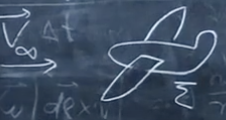
\includegraphics[width=0.2\textwidth]{14/pic_1.png}
	\caption{\label{ris:image14.1}}
\end{wrapfigure}

\begin{center}
	\textit{\underline{Примеры потенциалов.}}
\end{center}

Тут мы рассмотрим примеры различных функций $\varphi $. Рассматриваем задачу с набегающим с скоростью $\overrightarrow{v}_{\infty}$ однородным потоком на (как мы считаем покоящееся) тело.  Поверхность = $\Sigma$ и $\infty$  , т. о. $v_{\eta \leftarrow \infty} = v_\infty$ . Заметим, что задача линейная и потому складывая решения мы получим снова решение данной задачи.

1. Рассмотрим $\varphi_0 = \overrightarrow{v}_{\infty} x$, таким образом $grad \varphi = 0$ - все компоненты равны 0 . Это ситуация постоянного, однородного течения (течения на бесконечности). То , к чему стремится задача обтекания тела. Линии тока - прямые линии $z=y=const$

\begin{wrapfigure}{r}{0.2\textwidth}
	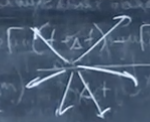
\includegraphics[width=0.2\textwidth]{14/pic_2.png}
	\caption{\label{ris:image14.2}}
\end{wrapfigure}

2. Рассмотрим $\varphi_1 = \frac{q}{r}, \ r = sqrt(x^2+y^2+z^2), \ q \ \text{это некоторая константа}$. Рассматриваем сферическую систему координат. Имеем в такой системе зависимость только от радиуса - имеем одну радиальную компоненту скорости $v_r = \frac {\partial \varphi_1 } {\partial r}= -\frac{\partial q}{\partial r^2}.$ Линии тока  на рисунке  2 - по напрвлению r $\theta = \varphi_1 = conts$. Если $q < 0$ это источник, если $q > 0$ это сток. $div \overrightarrow{v} = 0$, можем проинтегрировать по  сфере $Q = \int\limits_{S} \overrightarrow{v} d \overrightarrow{s} $ , получим $\varphi_1 =- \frac{Q}{4\Pi r}$

\begin{wrapfigure}{r}{0.2\textwidth}
	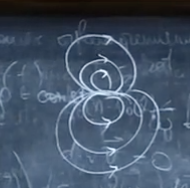
\includegraphics[width=0.2\textwidth]{14/pic_3.png}
	\caption{\label{ris:image14.3}}
\end{wrapfigure}

3. Можем рассмотреть $\varphi_2 = \frac{\partial \varphi_1} {\partial x}$.  Это диполь . Линии тока , получающиеся при данном потенциале, приведены на рисунке 3.


4. Можем сложить прошлые потенциалы и получить новый $\varphi_3 = \varphi_0 - \frac{\partial}{\partial x} \frac{Q}{4\Pi r}$. При некотором  $r$ данное выражение становится равно 0. Таким образом данный потенциал соответствует обтеканию шара

\newpage 

\begin{center}
	\textit{\underline{Примеры плоских течений. }}
	\\
	\textit{\underline{Применение теории функции комплексного
		 		переменного для решения задач плоского движения }}
	 \\
	 \textit{\underline{ идеальной несжимаемой жидкости. }}
\end{center}

Рассмотрим уравнение неразрывности в плоском случае 
$$
\frac{\partial u}{\partial x} + \frac{\partial v}{\partial y} = 0
$$
Уравнение отсутствия вихря 
$$
rot \overrightarrow{v} = 
\begin{vmatrix}
	\overrightarrow{e_x} & \overrightarrow{e_y}  & \overrightarrow{e_z} \\
	\frac{\partial }{\partial x} & \frac{\partial }{\partial y} & 0\\
	u & v & 0\
\end{vmatrix} = \overrightarrow{e_z} (\frac{\partial u}{\partial x} - \frac{\partial v}{\partial y} )
$$

\begin{wrapfigure}{r}{0.2\textwidth}
	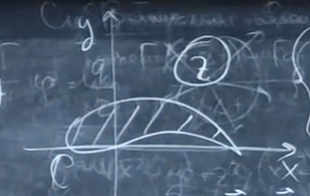
\includegraphics[width=0.2\textwidth]{14/pic_4.png}
	\caption{\label{ris:image14.4}}
\end{wrapfigure}

таким образом получаем условия Коши-Римана 
$$ \begin{cases}
\frac{\partial u}{\partial x} + \frac{\partial v}{\partial y} = 0  \ (\leftrightarrow \exists \psi)\\
\frac{\partial u}{\partial x} - \frac{\partial v}{\partial y}  = 0 \ (\leftrightarrow \exists \varphi)
\end{cases},$$

можем ввести комплескную переменную $x = x + i y$, т. о. $v = u + iv$, второе равенство из условий К-Р
$$ \begin{cases}
	\frac{\partial \varphi}{\partial x} = u  = \frac{\partial \psi}{\partial y}\\
	\frac{\partial \psi}{\partial y} = v = -\frac{\partial \varphi}{\partial x} 
\end{cases},$$
Таким образом получаем голоморфную функцию $w = \varphi + i \psi$. Если подставим в условие неразрывности , то получим $\Delta \varphi = 0$ , и при добавлении условия $\frac{\partial \varphi}{\partial n} |_C = 0 $ (условие непротекания), получим задачу Неймана. Здесь $C$ это просто контур.

В свою очередь если подставить $\psi $ в уравнение отсутствия вихря получим задачу Дирихле
$ \Delta \psi = 0 \quad \psi |_C = 0$



Рассмотрим дифференциал $d \psi$
$$
d \psi = \frac{\partial \psi}{\partial x}  dx +  \frac{\partial \psi}{\partial y}  dy = -vdx + udy
$$
\begin{wrapfigure}{r}{0.21\textwidth}
	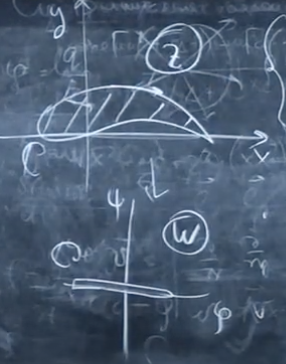
\includegraphics[width=0.21\textwidth]{14/pic_5.png}
	\caption{\label{ris:image14.5}}
\end{wrapfigure}
В свою очередь если $\psi = const $ (смысл линии - это линия тока), то $\frac{\partial x}{\partial u} = \frac{\partial y}{\partial v} $


Что такое \sout{бит}  функция w ? $w = \varphi x + i \psi$ - функция $z$, переводит конформно плоскость $z$ в плоскость $w$ , где $w=w(z)$ - комплексный потенциал течения

Во что перейдет контур $C$. По условию линия тока это константа. Пусть линия тока соответсвует $psi = q$, тогда контур в плоскости $w$ перейдет в отрезок (см. рисунок). То есть для решения задачи обтекания какого то плоского тела надо придумать функцию $w$, чтобы она сплющила тело до отрезка , лежащего на отрезке $\psi = 0$, на оси $\varphi$
$$$$
\newpage 

\begin{wrapfigure}{r}{0.15\textwidth}
	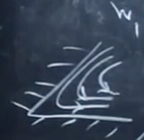
\includegraphics[width=0.15\textwidth]{14/pic_6.png}
	\caption{\label{ris:image14.6}}
\end{wrapfigure}



Рассмотрим каким течениям соответствуют какие  ситуации (потенциалы).

\begin{wrapfigure}{l}{0.15\textwidth}
	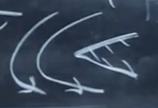
\includegraphics[width=0.15\textwidth]{14/pic_7.png}
	\caption{\label{ris:image14.7}}
\end{wrapfigure}

1. Однородное течение, $w_0 = \overline{v}_{\infty} z$  , где $ \overline{v}_{\infty}  = const$ . Что такое $w'$ ? Это голоморфная функция , поэтому $w' = \frac{\partial \varphi}{\partial x} + i \frac{\partial \psi}{\partial x}  = u - iv = \overline{v}$


$w_0^{'} = \overline{v}_{\infty}$. В каждой точке скорость = const и равна $v_{\infty}$

2. $w_1 = z^n = r^n e^{i \theta n} = r^n(\cos(n \theta) + i \sin (n \theta) )$.  

Линии тока это $r^n \sin(n \theta) = const $ 

Рис 6 : $n > 1$ , течение в таком углу 

Рис 7: обтекание угла при $n < 1$ \\

В данном случае можем применить , например , инверсию . Можем наоборот , прямые линии (из плоскости w) перейти в течение (плоскость z)

$$ \begin{cases}
	w  = \frac{\partial u}{\partial z}\\
	z = -\frac{\partial u}{\partial w} 
\end{cases},$$

С помощью данного преобразования прямые линии на $w$ перейдут в окружности на $z$ . Причем окружности будут проходить через ноль. На самом деле получится диполь - см. рисунок 3.  

3. $z = e^{q w}, \ q \in \mathbb{R} , \quad w = \varphi + i \psi$. Таким образом $z = e^{q \varphi} e^{i q \psi}$, при этом $e^{i q \psi} = const$, радиус при этом пробегаем все диагонали $\varphi$

 Если $z$ чисто мнимое , то получаем течение - вихри. Соответствует рисунку 2.
